%%%%%%%%%%%%%%%%%%%%%%
%%Options for presentations (in-class) and handouts (e.g. print). 
\documentclass[pdf
%,handout
]{beamer}
\usepackage{pgfpages}
%\pgfpagesuselayout{2 on 1}[letterpaper,border shrink=5mm]

\graphicspath{{../}}
%%%%%%%%%%%%%%%%%%%%%%
%% Change this for different slides so it appears in bar
\usepackage{authoraftertitle}
\date{6.1: Complex Numbers}

%%%%%%%%%%%%%%%%%%%%%%
%% Upload common style file
\usepackage{../LyryxLinearAlgebraSlidesStyle}

\usetikzlibrary{shapes, calc, shapes, arrows}
%\usepackage{amsmath,amssymb}

\usepackage{xcolor}
\definecolor{xvectorcolor}{HTML}{77933C}

\begin{document}
	
	%%%%%%%%%%%%%%%%%%%%%%%
	%% Title Page and Copyright Common to All Slides	
	%Title Page
	\input ../frontmatter/titlepage.tex	
	%LOTS Page
	%\input frontmatter/lyryxopentexts.tex	
	%Copyright Page
	\input ../frontmatter/copyright.tex	
	%%%%%%%%%%%%%%%%%%%%%%%%%

\section{Complex Numbers} 
%-------------- start slide -------------------------------%
{
\frame{
\begin{block}{ Why complex numbers?}
\begin{itemize}
\item Counting numbers: $1, 2, 3, 4, 5, \ldots$
\item<2-> Integers: $0, 1, 2, 3, 4 \ldots$ but also
$-1, -2, -3 \ldots$
\item<3->
To solve $3x+2=0$, integers aren't enough, 
so we have \alert{rational numbers} (fractions), i.e.,
\vspace*{-.2in}

\[ \mbox{if } 3x+2 = 0, \mbox{ then } x=-\frac{2}{3}.\]
\vspace*{-.2in}

\item<4-> 
We still can't solve $x^2-2=0$ because there are no rational
numbers $x$ with the property that $x^2-2=0$, so we have
\alert{irrational numbers}, i.e.,
\vspace*{-.2in}

\[ \mbox{if } x^2-2 = 0, \mbox{ then } x=\pm\sqrt{2}.\]
\vspace*{-.2in}

\item<5->
The set of \alert{real numbers}, $\RR$, consists of all
rational and irrational numbers (note that integers are
rational numbers).  However, we still can't solve
\vspace*{-.25in}

\[ x^2+1 = 0\]
\vspace*{-.2in}

because this requires $x^2=-1$, but any \alert{real} number
$x$ has the property that $x^2\geq 0$.
\end{itemize}
\end{block}
}}
%-------------- end slide -------------------------------%

%-------------- start slide -------------------------------%
\frame{\frametitle{Complex Numbers}
\begin{definitions}
\begin{itemize}
\item<2->
The \alert{imaginary unit}, denoted $i$, is defined to be
a number with the property that $i^2=-1$.
\item<3->
A \alert{pure imaginary} number has the form $bi$ where 
$b\in\RR$, $b\neq 0$, and $i$ is the imaginary unit.
\item<4->
A \alert{complex number} is any number $z$ of the form
\[ z = a + bi\]
where $a,b\in\RR$ and $i$ is the imaginary unit.
\begin{itemize}
\item<5->
$a$ is called the \alert{real part} of $z$.
\item<6->
$b$ is called the \alert{imaginary part} of $z$.
\item<7->
If $b=0$, then $z$ is a real number.
\end{itemize}
\end{itemize}
\end{definitions}
}
%-------------- end slide -------------------------------%

%-------------- start slide -------------------------------%
\frame{
\begin{block}{The Complex Plane (Argand Plane)}
\pause
A complex number $z=a+bi$ can be represented geometrically
by the point $(a,b)$ in the $xy$-plane, where
the $x$-axis is the \alert{real axis} and the $y$-axis is
the \alert{imaginary axis}.

\pause
\begin{picture}(3,2.1)
\put(1,0){\includegraphics[scale=.8]{figures/complex-plane.pdf}}
{\small
\put(1.25,0.2){$0$}
\put(2.8,0.2){$x$}
\put(1.23,1.6){$y$}
\put(2.5,1.2){$(a,b)$}}
{\footnotesize
\put(1.9,1.25){$a$}}
\put(2.45,0.8){$b$}
\end{picture}
\pause
\begin{itemize}
\item Real numbers: $a+0i$ lie on the $x$-axis.
\pause
\item Pure imaginary numbers: $0 + bi$ ($b\neq 0$) lie on
the $y$-axis.
\end{itemize}
\end{block}
}
%-------------- end slide -------------------------------%

%-----------------start slide------------------------------%
\frame{
\begin{block}{Addition and Subtraction of Complex Numbers}
\pause
Let $\textcolor{blue}{z=a+bi}$ and
$\textcolor{orange}{w=c+di}$ be complex numbers.
\pause
\begin{itemize}
\item
\alert{Equality}
$\textcolor{blue}{z}=\textcolor{orange}{w}$ if and
$\textcolor{blue}{a}=\textcolor{orange}{c}$ and
$\textcolor{blue}{b}=\textcolor{orange}{d}$.
\pause
\item
\alert{Addition}
\vspace*{-.1in}
\pause

\[ \textcolor{blue}{z} + \textcolor{orange}{w}
= \pause \textcolor{blue}{(a+bi)} + \textcolor{orange}{(c+di)}
= \pause  (\textcolor{blue}{a}+\textcolor{orange}{c})
+ (\textcolor{blue}{b}+\textcolor{orange}{d})i. \]
\vspace*{-.1in}

\pause
\item
\alert{Subtraction}
\vspace*{-.1in}
\pause

\[ \textcolor{blue}{z} - \textcolor{orange}{w}
= \textcolor{blue}{(a+bi)} - \textcolor{orange}{(c+di)}
=  (\textcolor{blue}{a}-\textcolor{orange}{c})
+ (\textcolor{blue}{b}-\textcolor{orange}{d})i. \]
\end{itemize}
\end{block}
\pause
\begin{examples}
\begin{itemize}
\item $(-3+6i) + (5-i) = \pause 2+5i$.
\pause
\item $(4-7i) + (6-2i) = \pause 10-9i$.
\pause
\item $(-3+6i) - (5-i) = \pause -8+7i$.
\pause
\item $(4-7i) - (6-2i) = \pause -2-5i$.
\end{itemize}
\end{examples}
}
%-------------- end slide -------------------------------%

%-----------------start slide------------------------------%
%-------------- end slide -------------------------------%

%-----------------start slide------------------------------%
%-------------- end slide -------------------------------%

%-----------------start slide------------------------------%
%-------------- end slide -------------------------------%

%-----------------start slide------------------------------%
\frame{
\begin{block}{Properties of Addition}
\pause
Let $z$, $w$, and $v$ be complex numbers.
\pause
\begin{enumerate}
\item $z + w = w + z$.
\hfill{\textcolor{blue}{(addition is commutative)}}
\medskip
\pause
\item $(z + w) + v = z + (w + v)$.
\hfill{\textcolor{blue}{(addition is associative)}}
\medskip
\pause
\item $z + 0 = z$.
\hfill{\textcolor{blue}{(existence of an additive identity)}}
\medskip
\pause
\item
For every $z=a+bi$ there exists a complex number $-z = -a -bi$ such that 
$z + (-z) = 0$.
\hfill{\textcolor{blue}{(existence of an additive inverse)}}
\end{enumerate}
\end{block}
}
%------------------------end slide--------------------------%


%-------------- start slide -------------------------------%
\frame{
\begin{block}{Addition in the Complex Plane}
\pause
If $z=a+bi$ and $w=c+di$, then $z+w=(a+c)+(b+d)i$.  
\pause
Geometrically, we have:
\bigskip

\begin{picture}(3,2)
\put(1.25,0){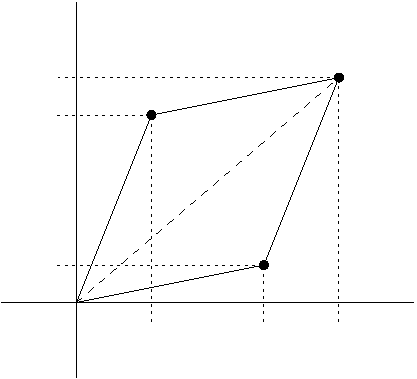
\includegraphics[scale=.75]{figures/addition.pdf}}
{\small
\put(1.5,0.25){$0$}
\put(3.2,0.25){$x$}
\put(1.5,1.75){$y$}
\put(2.65,0.54){$z$}
\put(1.93,1.40){$w$}
\put(3.00,1.50){$z+w$}
}
{\footnotesize
\put(1.98,0.20){$c$}
\put(2.53,0.20){$a$}
\put(2.81,0.20){$a+c$}
\put(1.45,0.55){$b$}
\put(1.45,1.30){$d$}
\put(1.22,1.48){$b+d$}
}
\end{picture}
\bigskip
\pause

$0$, $z$, $w$, and $z+w$ are the vertices of a parallelogram.
\end{block}
}
%-------------- end slide -------------------------------%

%---------------- start slide--------------------------%
\frame{
\begin{block}{Multiplication of Complex Numbers}
Let $z=a+bi$ and $w=c+di$ be complex numbers.
Then the \alert{product} of $z$ and $w$ is
\[ zw=(a+bi)(c+di) = (ac-bd)+(ad+bc)i.\]
\pause
\alert{The multiplication is done essentially as the product of
two linear polynomials, with $i^2$ replaced by $-1$.}
\end{block}
\medskip

\pause
\begin{example}
\vspace{-1em}
\begin{eqnarray*} 
(2-3i)(-3+4i) = &=& ((2)(-3) - (-3)(4))+((2)(4)+(-3)(-3))i \\
&=& (-6 + 12) + (8 + 9)i \\
&=& 6+17i
\end{eqnarray*}
\end{example}
}
%----------------------end slide--------------------------%

%-----------------------start slide-------------------%
\frame{
\begin{block}{Properties of Multiplication}
\pause
Let $z, w$ and $v$ be complex numbers.
\pause
\begin{itemize}
\item $zw=wz$.
\hfill{\textcolor{blue}{(multiplication is commutative)}}
\medskip
\pause
\item $(zw)v=z(wv)$.
\hfill{\textcolor{blue}{(multiplication is associative)}}
\medskip
\pause
\item $z (w+v) = zw + zv$.
\hfill{\textcolor{blue}{(multiplication distributes over addition)}}
\medskip
\pause
\item $1z=z$.
\hfill{\textcolor{blue}{(`1' is the multiplicative identity)}}
\medskip
\pause
\item
For each $z \neq 0$, there exists $z^{-1}$ such that
$z z^{-1} = 1$.\\ 
\hfill{\textcolor{blue}{(existence of a multiplicative inverse)}}
\end{itemize}
\end{block}
}
%---------------------------end slide---------------------%
%-------------- start slide -------------------------------%
\frame{
\begin{problem}\em
Find all complex numbers $z$ so that $z^2=-3+4i$.
\end{problem}
\pause
\begin{solution}\em
Let $z=a+bi$.  Then
\vspace*{-.15in}

\[ z^2=(a+bi)^2=(a^2-b^2)+2abi = -3+4i,\]
\vspace*{-.3in}

\pause
so 
\[ a^2-b^2=-3 \mbox{ and } 2ab=4.\]
\vspace*{-.25in}

\pause
Since $2ab=4$, $a=\frac{2}{b}$. 
\pause
Substituting this into
the first equation gives us
\pause
\begin{eqnarray*}
a^2-b^2 & = & -3 \\
\left(\frac{2}{b}\right)^2 - b^2 & = & -3 \\ \pause
\frac{4}{b^2} - b^2 & = & -3 \\ \pause
4- b^4 & = & -3b^2 \\ \pause
b^4-3b^2-4 & = & 0.
\end{eqnarray*}

\vspace*{-.1in}
\end{solution}
}
%-------------- end slide -------------------------------%

%-------------- start slide -------------------------------%
\frame{
\begin{solution}[continued]
Now, $b^4-3b^2-4=0$ can be factored \pause into
\begin{eqnarray*}
(b^2-4)(b^2+1)& = & 0\\
\pause
(b-2)(b+2)(b^2+1)& = & 0.
\end{eqnarray*}
\pause
Since $b\in \RR$ and $b^2+1$ has no real roots, $b=2$ or $b=-2$.
\bigskip
\pause

Since $a=\frac{2}{b}$, it follows that
\pause
\begin{itemize}
\item when $b=2$, $a=1$, and $z=a+bi=1+2i$;
\pause
\item when $b=-2$, $a=-1$, and $z=a+bi=-1-2i$.
\pause
\end{itemize}

\bigskip
Therefore, if $z^2=-3+4i$, then $z=1+2i$ or $z=-1-2i$.
\end{solution}
}
%-------------- end slide -------------------------------%

%-------------- start slide -------------------------------%
\frame{
\begin{block}{The Conjugate of a Complex Number}
\pause
Let $z=a+bi$ be a complex number.
\pause
The \alert{conjugate} of $z$ is the complex number
\alert{$\overline{z}=a-bi$}.
\pause
Geometrically, $\overline{z}$ is the reflection of $z$ in the $x$-axis.
\pause

\begin{picture}(3,1.27)
\put(1.2,0){\includegraphics[scale=.6]{figures/conjugate.pdf}}
{\footnotesize
\put(1.4,0.5){$0$}
\put(1.4,1.1){$y$}
\put(2.3,0.5){$x$}
\put(2.2,1.0){$(a,b)$}
\put(2.2,0.2){\alert{$(a,-b)$}}
}\end{picture}
\end{block}

\pause
\begin{examples}
\begin{itemize}
\pause
\item If $z=3+4i$, then $\overline{z}=\pause 3-4i$,
\pause
i.e., $\overline{3+4i}=3-4i$.
\pause
\medskip

\item $\overline{-2+5i}=\pause -2-5i$.
\pause
\medskip

\item $\overline{i}=\pause -i$.
\pause
\medskip

\item $\overline{7}=\pause 7$.
\end{itemize}
\end{examples}
}
%-------------- end slide -------------------------------%

%----------------------start slide-------------------%
\frame{
\begin{block}{Properties of the Conjugate}
Let $z$ and $w$ be complex numbers.
\begin{itemize}
\item
$\overline{z\pm w} = \overline{z} \pm \overline{w}$.
\pause
\item
$\overline{(zw)} = \overline{z}~ \overline{w}$.
\medskip
\pause
\item
$\overline{(\overline{z})}=z$.
\pause
\medskip
\item
$\overline{\left(\frac{z}{w}\right)} =
\frac{\overline{z}}{\overline{w}}$.
\pause
\medskip
\item
$z$ is real if and only if $\overline{z}=z$.
\end{itemize}
\end{block}
\pause
\begin{alertblock}{Note}
If $z=a+bi$, then
\pause
\[ z\overline{z}=
\pause
(a+bi)(a-bi)=
\pause
a^2 + b^2.\]
\end{alertblock}
}
%-------------------- end slide --------------------%

%-------------- start slide -------------------------------%
\frame{
Lecture 2
}
%-------------- end slide -------------------------------%

%-------------- start slide -------------------------------%
\frame{
\begin{block}{Division of Complex Numbers}
\pause
Let $z=a+bi$ and $w=c+di$ be complex numbers.
\pause
Suppose that $c,d$ are not both zero.
\pause
Then the \alert{quotient $z$ divided by $w$} is
\begin{eqnarray*}
\frac{z}{w}=
\pause
\frac{a+bi}{c+di} & = & \pause\frac{a+bi}{c+di}\times \frac{c-di}{c-di} \\
& = & \pause\frac{(ac+bd)+(bc-ad)i}{c^2+d^2} \\
& = & \pause\frac{ac+bd}{c^2+d^2} +\frac{bc-ad}{c^2+d^2}i.
\end{eqnarray*}
\pause
\alert{The quotient $\frac{z}{w}$ is obtained by multiplying
both top and bottom of $\frac{z}{w}$ by $\overline{w}$ and
then simplifying the expression.}
\end{block}
}
%-------------- end slide -------------------------------%

%-------------- start slide -------------------------------%
\frame{
\begin{examples}
\pause
\begin{itemize}
\item
\[ \frac{1}{i} = \pause \frac{1}{i}\times \frac{-i}{-i}
=\frac{-i}{-i^2}=-i. \]
\pause
\item
{\small
\[ \frac{2-i}{3+4i} = \pause \frac{2-i}{3+4i}\times \frac{3-4i}{3-4i}
=\frac{(6-4)+(-3-8)i}{3^2+4^2}
=\frac{2-11i}{25}
=\frac{2}{25} - \frac{11}{25}i. \]}
\pause
\item
{\small
\[ \frac{1-2i}{-2+5i} = \pause \frac{1-2i}{-2+5i}\times \frac{-2-5i}{-2-5i}
=\frac{(-2-10) + (4-5)i}{2^2+5^2}
=-\frac{12}{29}-\frac{1}{29}i.  \]}
\end{itemize}
\end{examples}
}
%-------------- end slide -------------------------------%



%---------------start slide--------------------------%
\frame{
\begin{block}{The Multiplicative Inverse}
Every nonzero complex number $z=a+bi$ has a unique
\alert{multiplicative inverse} $z^{-1}=\frac{1}{z}$ such that
$zz^{-1} = 1$, and 
\pause
\[ \frac{1}{z} =
\pause
\frac{1}{z}\times \frac{\overline{z}}{\overline{z}} =
\pause
\frac{\overline{z}}{z\overline{z}} =
\pause
\frac{a-bi}{a^2+b^2} =
\pause
\frac{a}{a^2+b^2}-\frac{b}{a^2+b^2}i.\]
\pause
\alert{Since $z$ is nonzero, $a^{2} + b^{2} \neq 0$, so the inverse is defined.}
\end{block}
\pause
\begin{example}
When $z = 2 + 6i$, $z^{-1}$ is defined, and
\pause
\[ \frac{1}{z}=
\frac{1}{2+6i} =
\pause
\frac{1}{2+6i}\times \frac{2-6i}{2-6i}=
\pause
\frac{2-6i}{2^2+6^2} =
\pause
\frac{2-6i}{40} =
\pause
\frac{1}{20} -  \frac{3}{20}i. \]
\pause
\alert{You can always check that $zz^{-1}=1$.}
\end{example}
}
%----------------end slide--------------------------%

%-------------- start slide -------------------------------%
\frame{\frametitle{Modulus}
\begin{block}{}
The \alert{absolute value} or \alert{modulus} of a complex
number $z=a+bi$ is 
\[ \left| z \right| = \sqrt{a^2+b^2}\]
\pause
{\em Note that this is consistent with the definition of the
absolute value of a real number.}
\medskip
\pause

Geometrically,  $|z|=\sqrt{a^2+b^2}$ is the distance from $z$ to the origin.

\begin{picture}(3,1.1)
\put(1.2,0){\includegraphics[scale=.6]{figures/absolute-value.pdf}}
{\footnotesize
\put(1.4,0.2){$0$}
\put(1.4,0.9){$y$}
\put(2.3,0.2){$x$}
\put(2.25,0.8){$(a,b)$}}
{\scriptsize
\put(1.8,0.2){$a$}
\put(2.25,0.5){$b$}}
{\tiny
\put(1.55,0.62){\alert{$\sqrt{a^2+b^2}$}}
}\end{picture}
\end{block}
}
%----------------end slide--------------------------%

%-------------- start slide -------------------------------%
\frame{
\begin{examples}
\pause
\begin{enumerate}
\item $|-3+4i|=
\pause
\sqrt{3^2+4^2}=
\pause \sqrt{25}=\pause 5$.
\pause

\medskip
\item $|3-2i|=\pause \sqrt{3^2+2^2}=\sqrt{13}$.
\pause

\medskip
\item $|i|=\pause \sqrt{1^2}=1$.
\end{enumerate}
\end{examples}
}
%-------------- end slide -------------------------------%

%-------------- start slide -------------------------------%
\frame{\frametitle{Properties of the Modulus}
\begin{block}{}
\pause
Let $z$ and $w$ be complex numbers.
\pause
\begin{enumerate}
\item
$z \cdot \overline{z} = |z|^2$.
\pause
\item
$\frac{1}{z}= \frac{\overline{z}}{|z|^2}$.
\pause
\item
$|z|\geq 0$ for all $z$.
\pause
\item
$|z|=0$ if and only if $z=0$.
\pause
\item
$|zw|=|z|~|w|$.
\pause
\item
$\left|\frac{z}{w}\right| =\frac{|z|}{|w|}$.
\pause
\item \textcolor{blue}{The Triangle Inequality}

$|z+w|\leq |z|+|w|$.
\end{enumerate}
\end{block}
}
%-------------- end slide -------------------------------%

%------------- start slide--------------------------------%
%\frame{\frametitle{The Triangle Inequality}
%
%The
%An important property of the modulus is called the \alert{triangle inequality}.
%
%\begin{theorem}\em
%Let $z,w$ be complex numbers. 
%
%\uncover<2->{
%The following two inequalities hold for any  complex numbers $z,w$:
%\begin{equation*}
%\begin{array}{l}
%\left| z+w\right| \leq \left| z\right| +\left| w\right|  \\
%\left| \left| z\right| -\left| w\right| \right| \leq \left| z-w\right| 
%\end{array}
%\end{equation*}}
%
%\uncover<3->{
%The first one is called the \alert{Triangle Inequality}.}
%\end{theorem}
%}
%---------------- end slide-----------------------------%

%-------------- start slide -------------------------------%
\frame{\frametitle{Distance in the plane}
\begin{block}{}
If $z=a+bi$ and $w=c+di$, then $|z-w|=\sqrt{(a-c)^2+(b-d)^2}$.
\pause

\begin{picture}(3,1.4)
\put(1.25,0){\includegraphics[scale=.5]{figures/difference.pdf}}
{\small
\put(1.35,0.1){$0$}
\put(2.4,0.1){$x$}
\put(1.35,1.15){$y$}
\put(1.85,1.05){$z=a+bi$}
\put(2.35,0.6){$w=c+di$}}
{\tiny
\put(1.35,1.0){$b$}
\put(1.35,0.6){$d$}
\put(1.51,0.8){$b-d$}
\put(1.9,0.55){$c-a$}
\put(1.73,0.1){$a$}
\put(2.23,0.1){$c$} }
\end{picture}
\bigskip

This shows that the \alert{distance} between 
$z$ and $w$ in the complex plane is just the absolute value
of their difference.
\end{block}
}
%-------------- end slide -------------------------------%

%-------------- start slide -------------------------------%
\frame{
	\begin{block}{The Triangle Inequality: Geometrically}
		Now consider the points $z$, $z+w$, and the origin $0$
		in the complex plane. These points may be considered as vectors in the plane:
		\pause
		
\begin{picture}(3.5,1.0)
\put(1.4,0){\includegraphics[scale=0.9]{figures/vectors-4.pdf}}
\put(1.5,0.3){$ w $}
\put(1.95,0.6){$z+w$}
\put(2.6,0.0){$z$}
\put(1.8,-0.1){$0$}
\end{picture}
 \vspace*{3mm}
 		
		The triangle formed by these points has sides of length $|z|$,
		and $|z+w|$ and $|w|$ (the absolute value of the difference
		between $z+w$ and $z$).
		\pause
		
		Since the length of \alert{any} side of a triangle is at most the
		sum of the lengths of the other two sides, we get
		\alert{$|z+w|\leq |z|+|w|$.}
	\end{block}
}
%-------------- end slide -------------------------------%



%%-------------- start slide -------------------------------%
%\frame{
%\begin{block}{The Triangle Inequality: Geometrically}
%Now consider the points $z$, $z+w$, and the origin $0$
%in the complex plane.
%\pause
%
%\begin{picture}(3,2)
%\put(1.25,0){\includegraphics[scale=.75]{figures/triangle-ineq.pdf}}
%{\small
%\put(1.9,0.25){$0$}
%\put(3.0,0.25){$x$}
%\put(2.05,1.75){$y$}
%\put(1.28,1.78){$z+w$}
%\put(2.85,0.73){$z$}}
%{\tiny
%\put(1.40,0.95){$|z+w|$}
%\put(2.10,1.27){$|w|$}
%\put(2.25,0.62){$|z|$}
%}
%\end{picture}
%\pause
%
%The triangle formed by these points has sides of length $|z|$,
%and $|z+w|$ and $|w|$ (the absolute value of the difference
%between $z+w$ and $z$).
%\pause
%
%Since the length of \alert{any} side of a triangle is at most the
%sum of the lengths of the other two sides, we get
%\alert{$|z+w|\leq |z|+|w|$.}
%\end{block}
%}
%%-------------- end slide -------------------------------%


\end{document}
